\section{DOMÓTICA}

El término domótica proviene de la unión de las palabras \emph{domus} (que significa casa en latín) y \emph{tica} (de automática, palabra en griego). La Real Academa Española lo define como el <<conjunto de sistemas que automatizan las diferentes instalaciones de una vivienda>>.

En este proyecto se utilizará el concepto de domótica como la tecnología aplicada al Internet de las Cosas en el hogar, es decir, conectar nuestro hogar a la nube.

\subsection{Historia}

\parpic[r][]{
    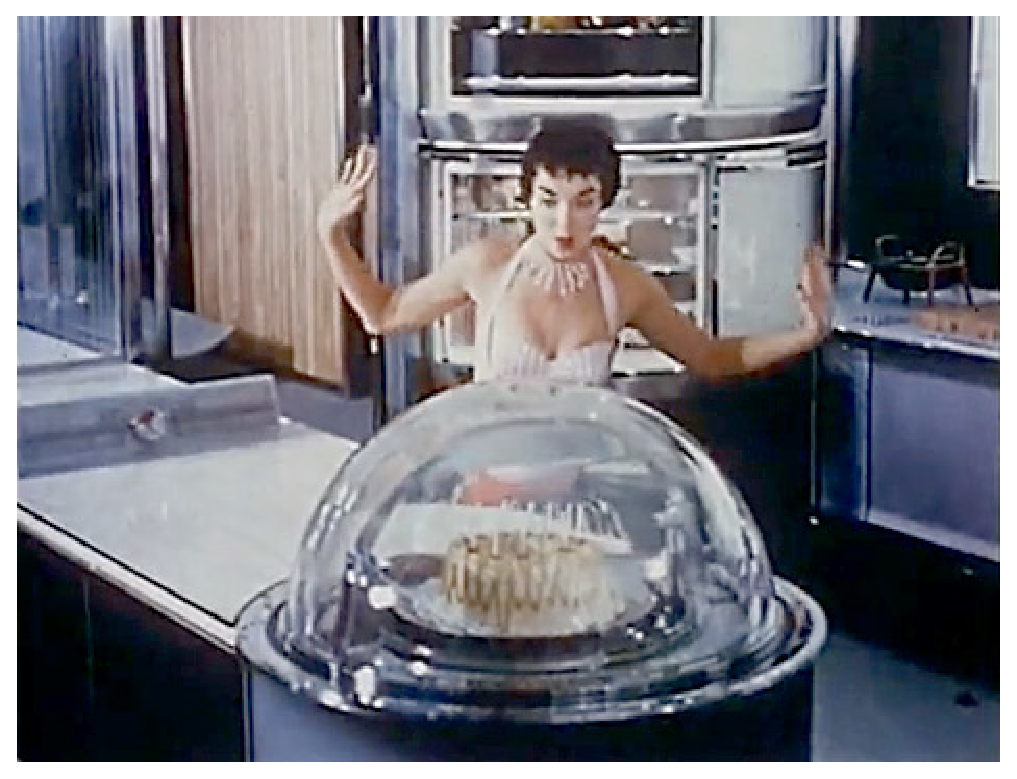
\includegraphics[keepaspectratio,width=0.25\textwidth]{Design_for_Dreaming_-_Cake_Under_Glass.eps}
    \label{fig:design-for-dreaming}
}

El hogar inteligente y automático comenzó a imaginarse en historias de ciencia ficción a inicios del siglo XX. En 1956 se emitió la película \emph{Design for Dreaming}~\ref{fig:design-for-dreaming} donde una mujer cae dormida y tiene una serie de sueños futuristas, incluyendo a \emph{Frigidaire}, la cocina automatizada del futuro. De ahí que no se pueda establecer una fecha concreta donde establecer el inicio de la domótica.

No obstante, si hemos de establecer una fecha de importante tenemos que hablar de 1975 con la aparición de \emph{X10}, un protocolo de comunicación que básicamente permite el control de las luces del hogar, para ello, utiliza la línea eléctrica como medio de comunicación. Debido a las limitaciones del protocolo de comunicación\emph{X10} se han desarrollado nuevas tecnologías para suplir estas carencias; CEBus, EIB, KNX...

A continuación se va a dar una breve explicación de cada una de estas tecnologías existentes en el mercado.

\subsection{X10}

\emph{X10} es un protocolo de comunicación para el control remoto de dispositivos eléctricos. Fue desarrollado en 1978 por \emph{Pico Electronics of Glenrothes}, Escocia, siendo la primera tecnología domótica en aparecer.

\parpic[r][]{
    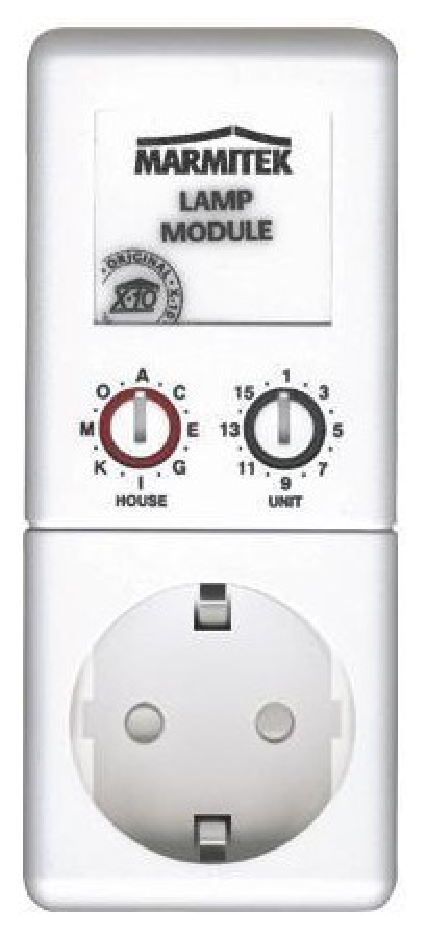
\includegraphics[keepaspectratio,width=0.09\textwidth]{modulo-lampara-x10.eps}
    \label{fig:modulo-lampara-x10}
}

Utiliza el cableado eléctrico como medio de comunicación que, debido a la limitación en ancho de banda que proporciona, solo es capaz de soportar hasta 256 dispositivos. A pesar de ello, es una tecnología ampliamente utilizada en Norteamérica y Europa por su característica de autoinstalable, sin necesidad de cableado adicional.

Las señales de control de X10 se basan en la transmisión de ráfagas de pulsos de \emph{RF} (120 kHz) que representan información digital. Estos pulsos se sincronizan en el cruce por cero de la señal de red (50 Hz ó 60 Hz). Con la presencia de un pulso en un semiciclo y la ausencia del mismo en el semiciclo siguiente se representa un '1' lógico y a la inversa se representa un '0'. A su vez, cada orden se transmite 2 veces, con lo cual toda la información transmitida tiene cuádruple redundancia. Cada orden involucra 11 ciclos de red (220 ms para 50 Hz y 183,33, para 60Hz).

Primero se transmite una orden con el Código de Casa y el Número de Módulo que direccionan el módulo en cuestión. Luego se transmite otro orden con el código de función a realizar (Function Code).

A continuación se muestra la tabla con los códigos que soporta el protocolo:

\begin{table}[!hbt]
    \begin{center}
        \begin{tabular}{|l |l | c | c |}
            \hline
            Código & Función & Unidireccional & Bidireccional \\
            \hline
            0 0 0 0 & All units off & X &  \\
            \hline
            0 0 0 1 & All lights on & X &  \\
            \hline
            0 1 1 0 & All lights off & X &  \\
            \hline
            0 0 1 0 & On & X &  \\
            \hline
            0 0 1 1 & Off & X &  \\
            \hline
            0 1 0 0 & Dim & X &  \\
            \hline
            0 1 0 1 & Bright & X &  \\
            \hline
            0 1 1 1 & Extended code & & X \\
            \hline
            1 0 0 0 & Hail request & & X \\
            \hline
            1 0 0 1 & Hail acknowledge & & X \\
            \hline
            1 0 1 0 & Pre-set dim & & X \\
            \hline
            1 1 0 1 & Status is on & & X \\
            \hline
            1 1 1 0 & Status is off & & X \\
            \hline
            1 1 1 1 & Status request & & X \\
            \hline
        \end{tabular}
        \caption{Listado de comandos \emph{X10}}
    \end{center}
\end{table}

\subsection{CEBus}

CEBus

\subsection{EIB}

EIB

\subsection{KNX}

KNX